\documentclass[a4paper,english,10pt]{article}\usepackage[]{graphicx}\usepackage[]{color}
%% maxwidth is the original width if it is less than linewidth
%% otherwise use linewidth (to make sure the graphics do not exceed the margin)
\makeatletter
\def\maxwidth{ %
  \ifdim\Gin@nat@width>\linewidth
    \linewidth
  \else
    \Gin@nat@width
  \fi
}
\makeatother

\definecolor{fgcolor}{rgb}{0.345, 0.345, 0.345}
\newcommand{\hlnum}[1]{\textcolor[rgb]{0.686,0.059,0.569}{#1}}%
\newcommand{\hlstr}[1]{\textcolor[rgb]{0.192,0.494,0.8}{#1}}%
\newcommand{\hlcom}[1]{\textcolor[rgb]{0.678,0.584,0.686}{\textit{#1}}}%
\newcommand{\hlopt}[1]{\textcolor[rgb]{0,0,0}{#1}}%
\newcommand{\hlstd}[1]{\textcolor[rgb]{0.345,0.345,0.345}{#1}}%
\newcommand{\hlkwa}[1]{\textcolor[rgb]{0.161,0.373,0.58}{\textbf{#1}}}%
\newcommand{\hlkwb}[1]{\textcolor[rgb]{0.69,0.353,0.396}{#1}}%
\newcommand{\hlkwc}[1]{\textcolor[rgb]{0.333,0.667,0.333}{#1}}%
\newcommand{\hlkwd}[1]{\textcolor[rgb]{0.737,0.353,0.396}{\textbf{#1}}}%
\let\hlipl\hlkwb

\usepackage{framed}
\makeatletter
\newenvironment{kframe}{%
 \def\at@end@of@kframe{}%
 \ifinner\ifhmode%
  \def\at@end@of@kframe{\end{minipage}}%
  \begin{minipage}{\columnwidth}%
 \fi\fi%
 \def\FrameCommand##1{\hskip\@totalleftmargin \hskip-\fboxsep
 \colorbox{shadecolor}{##1}\hskip-\fboxsep
     % There is no \\@totalrightmargin, so:
     \hskip-\linewidth \hskip-\@totalleftmargin \hskip\columnwidth}%
 \MakeFramed {\advance\hsize-\width
   \@totalleftmargin\z@ \linewidth\hsize
   \@setminipage}}%
 {\par\unskip\endMakeFramed%
 \at@end@of@kframe}
\makeatother

\definecolor{shadecolor}{rgb}{.97, .97, .97}
\definecolor{messagecolor}{rgb}{0, 0, 0}
\definecolor{warningcolor}{rgb}{1, 0, 1}
\definecolor{errorcolor}{rgb}{1, 0, 0}
\newenvironment{knitrout}{}{} % an empty environment to be redefined in TeX

\usepackage{alltt}
\usepackage{a4a}
%\VignetteIndexEntry{Introduction to a4a}
%\VignetteEngine{knitr::knitr}
\IfFileExists{upquote.sty}{\usepackage{upquote}}{}
\begin{document}

\title{Assessment for All initiative(a4a) \\ Introduction to FLa4a}

\author[1]{Ernesto Jardim}
\author[1,2,3]{Colin Millar}
\author[1]{Finlay Scott}
\author[1]{Chato Osio}
\author[1]{Iago Mosqueira}
\affil[1]{European Commission, Joint Research Centre, Sustainable resources directorate, Water and Marine Resources unit, 21027 Ispra (VA), Italy}
\affil[2]{Marine Scotland Freshwater Laboratory, Faskally, Pitlochry, Perthshire PH16 5LB, UK}
\affil[3]{International Council for the Exploration of the Sea (ICES), H. C. Andersens Boulevard 44-46, 1553 Copenhagen V, Denmark}
\affil[*]{Corresponding author \href{mailto:ernesto.jardim@jrc.ec.europa.eu}{ernesto.jardim@jrc.ec.europa.eu}}



\maketitle
\tableofcontents
\newpage

\section{Background}

(This section is based on \href{http://icesjms.oxfordjournals.org/content/early/2014/04/03/icesjms.fsu050.abstract}{Jardim, et.al, 2014})

The volume and availability of data useful for fisheries stock assessment is continually increasing. Time series of 'traditional' sources of information, such as surveys and landings data are not only getting longer, but also cover an increasing number of species.

For example, in Europe the 2009 revision of the Data Collection Regulation (EU, 2008a) has changed the focus of fisheries sampling programmes away from providing data for individual assessments of 'key' stocks (i.e. those that are economically important) to documenting fishing trips, thereby shifting the perspective to a large coastal monitoring programme. The result has been that data on growth and reproduction of fish stocks are being collected for more than 300 stocks in waters where the European fleets operate.

Recognizing that the context above required new methodological developments, the European Commission Joint Research Centre (JRC) started its 'Assessment for All' Initiative (\aFa), with the aim to develop, test, and distribute methods to assess a large numbers of stocks in an operational time frame, and to build the necessary capacity/expertise on stock assessment and advice provision. 

The long-term strategy of \aFa is to increase the number of stock assessments while simultaneously promoting the inclusion of the major sources of uncertainty in scientific advice. Our aim is to reduce the required workload by developing a software framework with the methods required to run the analysis a stock assessment needs, including methods to deal with recognized bottlenecks, \emph{e.g.} model averaging to deal with model selection (\href{http://icesjms.oxfordjournals.org/content/early/2014/03/31/icesjms.fsu043.abstract}{Millar, et.al, 2014}). Moreover, we aim to make the analysis more intuitive, thereby attracting more experts to join stock assessment teams. Having more scientists/analysts working in fisheries management advice will increase the human resource basis, which is currently recognized to be limited. Regarding the former, \aFa promotes a risk analysis approach to scientific advice through a wider usage of Operating Model/\MSE approaches. We're focused on developing methods that can deal with the most common settings these type of analysis require, and creating the conditions for scientists to develop their own methods. Our expectation is that having a common framework, with clear data structures and workflows, will promote research in this area and make it simpler to implement and share methods.

To achieve these objectives, the Initiative identified a series of tasks, which were or are being carried out, namely:
\begin{itemize}
	\item define a moderate data stock;
	\item develop a stock assessment framework;
	\item develop a forecasting algorithm based on \MSE;
	\item organize training courses for marine scientists.
\end{itemize}

\section{License, documentation and development status}

The software is released under the \href{https://joinup.ec.europa.eu/community/eupl/home}{EUPL 1.1}.

For more information on the \aFa methodologies refer to \href{http://icesjms.oxfordjournals.org/content/early/2014/04/03/icesjms.fsu050.abstract}{Jardim, et.al, 2014}, \href{http://icesjms.oxfordjournals.org/content/early/2014/03/31/icesjms.fsu043.abstract}{Millar, et.al, 2014} and \href{http://journals.plos.org/plosone/article?id=10.1371/journal.pone.0154922}{Scott, et.al, 2016}.

Documentation can be found at \url{http://flr-project.org/FLa4a}. You are welcome to:

\begin{itemize}
	\item Submit suggestions and bug-reports at: \url{https://github.com/flr/FLa4a/issues}
	\item Send a pull request on: \url{https://github.com/flr/FLa4a/}
	\item Compose a friendly e-mail to the maintainer, see `packageDescription('FLa4a')`
\end{itemize}




\subsection{The moderate data stock}

The moderate data stock definition was an important step in the Initiative's development. It clearly focused the Initiative on stocks with some information, moving away from the data-poor stocks, but without moving into data rich methodologies. It was recognized that there is a lot of research at both extremes of the data availability spectrum, but comparatively little in the middle 'region'. From this came the idea of the 'moderate data stock'. 

The 'moderate data stock' constitutes the entry level of our analysis. It has at least the following available data, which can be assembled in different ways, using distinct methods.
 
\begin{itemize}
	\item in relation to exploitation:
	\begin{itemize}
		\item volume of catches, which may be split into landings and discards if possible;
		\item length frequencies of the catches, landings or discards;
		\item nominal effort (optional, needed in case CPUE indices are to be derived);
	\end{itemize}
	\item in relation to biology:
	\begin{itemize}
		\item estimated maturity ogive (e.g. can be as simple as an estimate of $L_{50}$);
		\item estimated growth model and parameters;
		\item estimated length-weight relationship;
	\end{itemize}
	\item in relation to abundance:
	\begin{itemize}
		\item index of abundance.
	\end{itemize}	
\end{itemize}

\subsection{The stock assessment framework}

The stock assessment model framework is a non-linear catch-at-age model implemented in \pkg{R}/\pkg{FLR}/\pkg{ADMB} that can be applied rapidly to a wide range of situations with low parametrization requirements. Later we'll come back to these characteristics and it's application (see vignette on sca).

\subsection{MSE}

The \MSE is a sophisticated simulation/forecasting algorithm that takes into account structural uncertainty about stock dynamics (growth, recruitment, maturity) and on exploitation by commercial fleets (selectivity), embedding the framework of decision making. 

The \aFa approach to \MSE is to develop a set of methods to build a standard algorithm, which has the most common elements of uncertainty and management. So that the development of the quantitative side of a \MSE can be done in a operational time frame.

\section{The \aFa approach to stock assessment and management advice}

As stated before, one of the main objectives of \aFa is to promote a risk type of analysis, so that scientific advice provides policy and decision makers a perspective of the uncertainty existing on stock assessments and its propagation into the scenarios being analyzed.

The sources of uncertainty implemented so far are related with the processes of growth, natural mortality and reproduction (stock-recruitment); and with the estimation of population abundance and fishing mortality by the stock assessment model. In all cases the framework can include sampling error.

The approach is split into 4 steps: (i) converting length data to age data using a growth model, (ii) modeling natural mortality, (iii) assessing the stock, and (iv) \MSE\footnote{Under development, to be released with version 2.0}.

These steps may be followed in sequence or independently, depending on the user's preferences. All that is needed is to use the objects provided by the previous step and provide the objects required by the next, so that data flows between steps smoothly. One can make the analogy with building with Lego, where for each layer the builder may use the pieces provided by a particular boxset, or make use of pieces from other boxsets. Figure \ref{fig:inout} shows the process, including the class of the objects that carry the data (in black).

\begin{figure}[H]
\centering
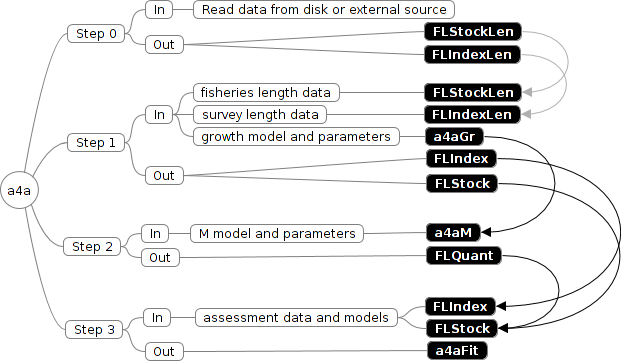
\includegraphics[width=\textwidth]{./inout}
\caption{In/out process of the \aFa approach. The boxes in black represent the classes of the objects that carry the information in and out of each step.}
\label{fig:inout}
\end{figure}

Analysis related to projections and biological reference points are dealt with by the \pkg{FLR} packages \pkg{FLash} and \pkg{FLBRP}. As such the Initiative does not provide specific methods for these analyses.

In Steps 1 and 2 there is no fitting of growth models or natural mortality models. The rationale is to provide tools that allow the uncertainty associated with these processes to be carried on into the stock assessment, e.g. through parameter uncertainty. This approach allows the users to pick up the required information from other sources of information such as papers, PhDs, Fishbase, other stocks, etc. If the stock under analysis does not have specific information on the growth or natural mortality processes, generic information about life history invariants may be used such as the generic priors suggested by \href{http://icesjms.oxfordjournals.org/content/early/2014/03/04/icesjms.fsu023.abstract}{Bentley, (2014)}.

Note that an environment like the one distributed by \aFa promotes the exploration of different models for each process, giving the analyst a lot of flexibility. It also opens the possibility to efficiently include distinct models in the analysis. For example, a stock assessment using two growth, or several models for natural mortality could be performed. Our suggestion to streamline the assessment process is to combine the final outcomes using model averaging (\href{http://icesjms.oxfordjournals.org/content/early/2014/03/31/icesjms.fsu043.abstract}{Miller, et. al, 2014}). Other solutions may be implemented, like scenario analysis, etc. What is important is to keep the data flowing smoothly and the models clear. R (\href{http://www.R-project.org/}{R Core Team, 2014}) and \pkg{FLR} (\href{http://icesjms.oxfordjournals.org/content/64/4/640.abstract}{Kell, et.al, 200}) provide powerful platforms for this approach.

%% ======================================
%% Call child document with libs and data

\section{Installing and loading libraries}

To run the \pkg{FLa4a} methods the reader will need to install the package and its dependencies and load them. Some datasets are distributed with the package and as such need to be loaded too.

\begin{knitrout}
\definecolor{shadecolor}{rgb}{0.969, 0.969, 0.969}\color{fgcolor}\begin{kframe}
\begin{alltt}
\hlcom{# from CRAN}
\hlkwd{install.packages}\hlstd{(}\hlkwd{c}\hlstd{(}\hlstr{"copula"}\hlstd{,}\hlstr{"triangle"}\hlstd{,} \hlstr{"coda"}\hlstd{))}
\hlcom{# from FLR}
\hlkwd{install.packages}\hlstd{(}\hlkwd{c}\hlstd{(}\hlstr{"FLCore"}\hlstd{,} \hlstr{"FLa4a"}\hlstd{),} \hlkwc{repos}\hlstd{=}\hlstr{"http://flr-project.org/R"}\hlstd{)}
\end{alltt}
\end{kframe}
\end{knitrout}

\begin{knitrout}
\definecolor{shadecolor}{rgb}{0.969, 0.969, 0.969}\color{fgcolor}\begin{kframe}
\begin{alltt}
\hlcom{# libraries}
\hlkwd{library}\hlstd{(devtools)}
\hlkwd{library}\hlstd{(FLa4a)}
\hlkwd{library}\hlstd{(XML)}
\hlkwd{library}\hlstd{(reshape2)}
\hlkwd{library}\hlstd{(latticeExtra)}
\hlcom{# datasets}
\hlkwd{data}\hlstd{(ple4)}
\hlkwd{data}\hlstd{(ple4.indices)}
\hlkwd{data}\hlstd{(ple4.index)}
\hlkwd{data}\hlstd{(rfLen)}
\end{alltt}
\end{kframe}
\end{knitrout}

\begin{knitrout}
\definecolor{shadecolor}{rgb}{0.969, 0.969, 0.969}\color{fgcolor}\begin{kframe}
\begin{alltt}
\hlkwd{packageVersion}\hlstd{(}\hlstr{"FLCore"}\hlstd{)}
\end{alltt}
\begin{verbatim}
## [1] '2.6.9.9007'
\end{verbatim}
\begin{alltt}
\hlkwd{packageVersion}\hlstd{(}\hlstr{"FLa4a"}\hlstd{)}
\end{alltt}
\begin{verbatim}
## [1] '1.6.2'
\end{verbatim}
\end{kframe}
\end{knitrout}



\section{How to read this document}

The target audience for this document are readers with some experience in R and some background on stock assessment.

The document explains the approach being developed by \aFa for fish stock assessment and scientific advice. It presents a mixture of text and code, where the first explains the concepts behind the methods, while the last shows how these can be run with the software provided. Moreover, having the code allows the reader to copy/paste and replicate the analysis presented here.

The sections and subsections are as independent as possible, so it can be used as a reference document for the \pkg{FLa4a}. 

%Section~\ref{sec:in} deals with reading and preparing data in \pkg{FLR} objects, which constitute the basic dataset for stock assessment with length structured models. This section is independent from \pkg{FLa4a} and relies mostly on \R and \pkg{reshape}.

%Sections~\ref{sec:l2a},\ref{sec:M} and \ref{sec:sca} are related with \pkg{FLa4a} and describe the concepts described in the previous section.

Finally, this is a live document which will be updated and released often.



\end{document}




